\chapter[Methodology]{Methodology}
\label{Chapter:Methodology}

% Work Objective 
In this work, we propose a methodology focused on domain partitioning and grouping that aims to reduce the computational workload and time consumed if we were to train a model on each point of a spatio-temporal domain. We argue that, by considering several models generated over representative elements of the domain, which generalize the temporal dimension of neighboring elements, it is possible to preserve a predictive quality comparable to the baseline approach of using a model for every element. As a result of applying the proposed methodology, we could process a spatio-temporal predictive query efficiently while maintaining a low error margin in the prediction.

% Methodology description
The process described by the methodology is divided into two phases, offline and online.The offline phase comprises two steps: (1) the domain partitioning, based on time-series clustering techniques; and (2) the construction of predictive models at each group representative sequence. The online phase is applied when processing a spatio-temporal predictive query, it consists of: (3) a process to select a set of pre-trained representative models, to schedule and run them; and (4) an approach to compose the query output using the forecasts of models allocated to every query region point. The methodology is represented by Figure \ref{Fig:OverviewMethodology}. The two main phases are shown in green, the steps for each phase in blue, the tasks performed in every step of the workflow in black, and finally, the corresponding expected products and outputs are shown in red. 

%The offline phase comprises three steps: (1) the domain partitioning process, based on clustering techniques, to find representative elements; (2) the generation of predictive models for the representatives; and (3) a model composition process to predict a subset of the domain region. The online phase consists of (4) a mechanism to compute a spatio-temporal predictive query. 

\begin{figure}[ht]
	\centering
	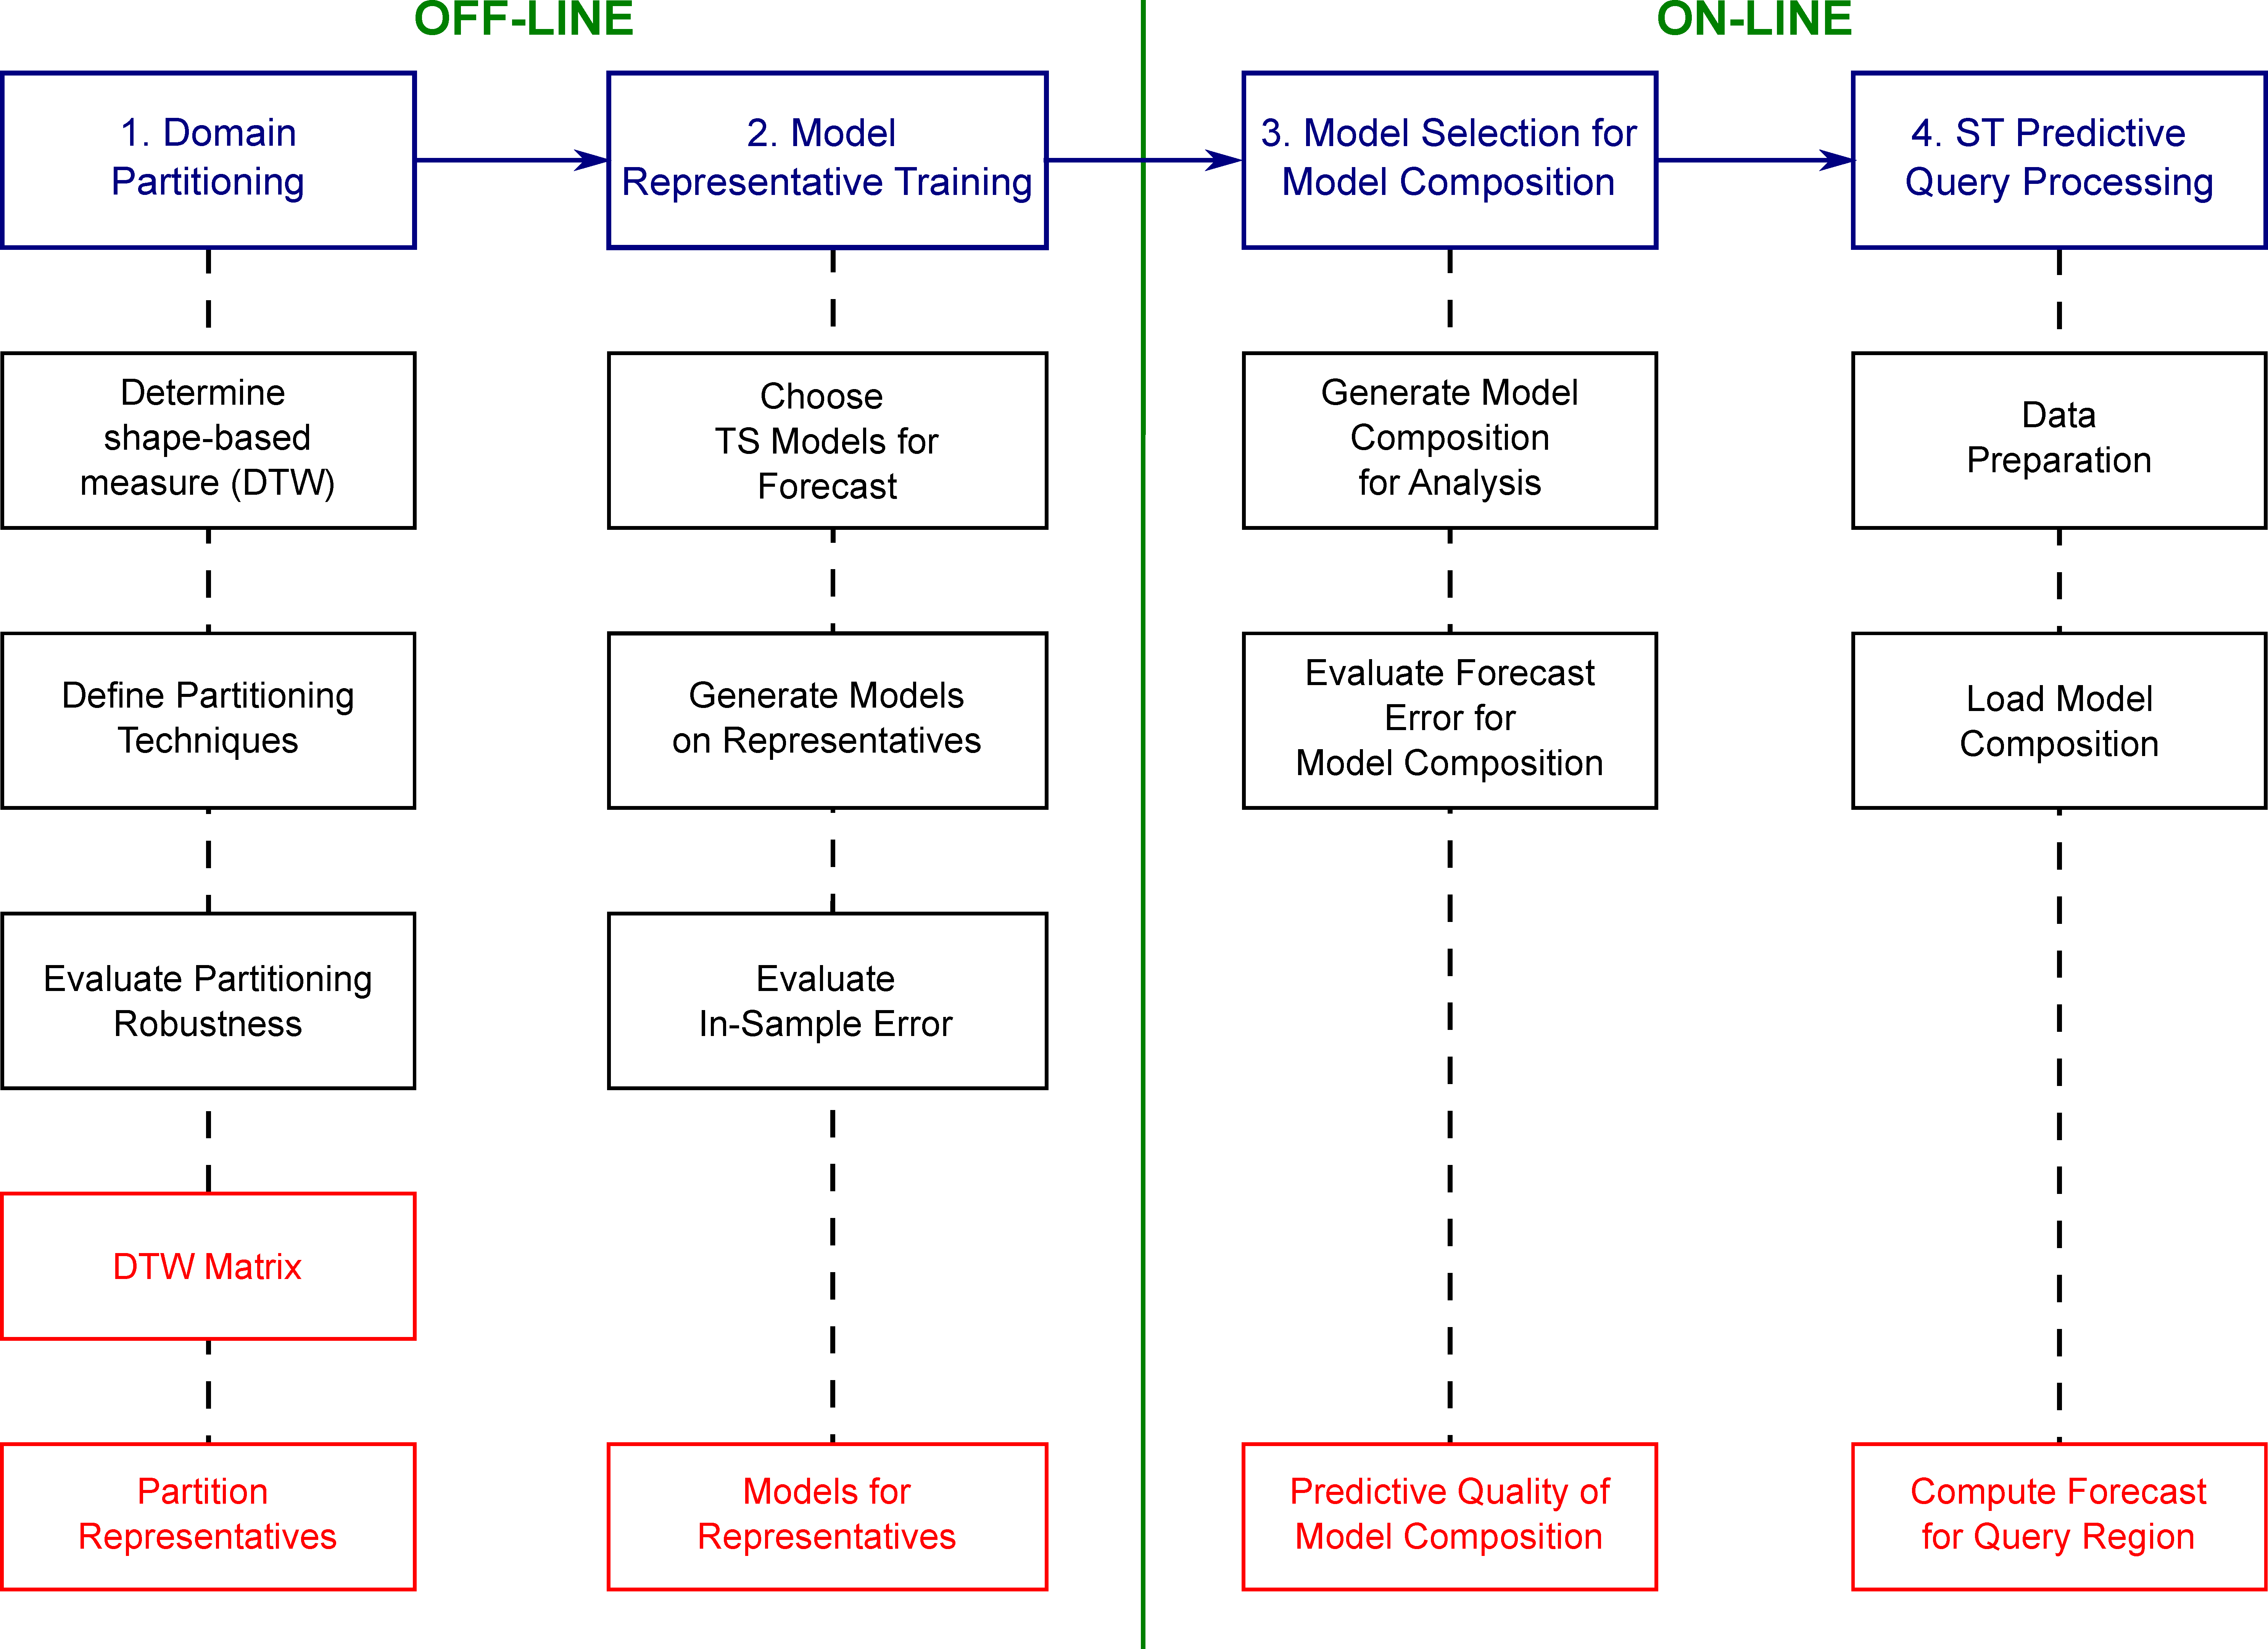
\includegraphics[scale=0.16]{../Figures/Methodology_Corrections}
	\caption{Workflow for the proposed methodology.}
	\label{Fig:OverviewMethodology}
\end{figure}

In Sections \ref{Sec:DomainPartitioning} to \ref{Sec:SpatioTemporalQueryProcessing}, we detail the tasks performed in each step, describing the tools and methods used as well as techniques to validate their performance. The last section discusses the decisions adopted during the development of the methodology.

\section{Step 1: Domain Partitioning}
\label{Sec:DomainPartitioning}

% Objective and general description
The purpose of this step is to i) find groups with high similarity according to the temporal evolution on a spatio-temporal domain (in particular univariate time-series) and ii) find representatives for each aforementioned group. We adopt clustering techniques to partition the domain by grouping elements based on a shape similarity measure. 

% Consider a representative element
We consider two methods for grouping elements that involve obtaining a representative element (which also exists on the domain) for each group. A representative is then said to generalize the temporal dimension of the other elements in the group. It is important to remember that in a clustering algorithm, the number of clusters, the size of clusters, the definition for outliers, and the definition of the similarity among the univariate time-series are all the concepts that depend on the problem (case study) at hand \cite{Aghabozorgi2015}.

For univariate time-series data, we use a shape-based similarity measure in order to leverage similarities in the temporal behavior of the spatio-temporal domain. In particular, we use Dynamic Time Warping (DTW), previously described in Section \ref{sec:ShapeBasedDistance}.

% What are the products
As part of the off-line process, we calculate the distance matrix quantifying the DTW similarity between any two time series on the domain. This process can demand considerable computational power, but efficient calculation is possible using data parallelism by calculating pairwise distances independently and in parallel. Additionally, the distance matrix only needs to be calculated once per domain dataset and saved into persistent storage for future lookups.

In this work, we consider the following techniques for domain partitioning:

\begin{itemize}%[noitemsep,nolistsep]		
	\item $k$-medoids clustering: the purpose of this technique is to group the domain elements that have a high degree of similarity (See Section \ref{Sec:kMedoidsClustering}). As mentioned before, we consider DTW as the similarity measure. 
	
	The benefits of using $k$-medoids as a clustering algorithm are two-fold. In addition to finding the groups that help minimize local dissimilarity, the algorithm returns a medoid for each group, an existing object. For our methodology, we can leverage the model trained on each medoid and measure the generalization error of this model when applied to other points in the corresponding cluster. A downside of the $k$-medoids approach is that it requires the computation of the distances between many points, which can have order of time complexity $O(n^2)$. To mitigate this problem, we can leverage a previously calculated distance matrix, which can be reused for all $k$-medoids clusters for that region, thereby significantly reducing the time to compute each $k$-medoids partitioning.
	
	\item Regular or naive partitioning: The spatio-temporal domain is first divided into $k$ rectangles of the same shape (allowing for irregularities when the dimensions cannot be exactly divided), and then, for each given group, we find the element (centroid) that minimizes the total sum of DTW distances to that element. This grouping is used as a baseline in our methodology to assess the adequacy of $k$-medoids better. This partitioning has no parameters besides the desired number of groups.
\end{itemize}

% Representation of partition profile using the problem formalization
Considering our formal representation in Section \ref{Sec:ProblemFormalization}, we can express the domain grouping for the spatio-temporal domain $\mathcal{D}$ as follows:

\begin{equation}
\mathcal{D} = \bigcup_{i=1}^{n} \mathbf{S}_{i},
\end{equation}
where for any $i\neq j$ we have that $\mathbf{S}_{i} \cap \mathbf{S}_{j} = \emptyset$, due to the crisp clustering algorithm. And for $\mathbf{S}_{i}$, we admit that a $\mathcal{S}_{i}^{*} \in \mathbf{S}_{i}$ exists (the representative of the group) such that generalizes the temporal dependence of all the elements in $\mathbf{S}_{i}$.

As mentioned in Section \ref{Sec:kMedoidsClustering}, there is the important issue of choosing the number of clusters $k$, which has been recognized as one of the vital issues essential to the success of clustering applications \cite{Aggarwal2013}. Unfortunately, despite the vast amount of expert efforts spent on this matter, there is no consistent and conclusive solution to cluster validation. We will explore some of the available techniques below on how they are applied to time series clustering.

\subsection{Determining the number of groups}
\label{Sec:domain_number_groups}

The performance of the $k$-Medoids algorithm is dependent on the optimal value of $k$, the number of clusters to be generated. The $k$-medoids algorithm requires the user to specify the value of $k$, and finding a suitable value is very challenging for time series data set. The choice is often ambiguous, with interpretations depending on the shape and scale of the distribution of the time series in a dataset \cite{Liao2005}. An optimal choice of $k$ should strike a balance between maximizing the compression of the data using a single cluster while maximizing the accuracy when assigning each data point to its cluster. Here, we explore some of the available methods for finding a suitable value for $k$.

When using a clustering technique for high volumes of data and low variability of the data values throughout neighbor points, it is difficult to determine the optimal number of groups ($k$). It is particularly important for our problem, where there is low variation in the spatial data distribution of the different time series. To identify a cluster in a dataset, we try to minimize the distance between points in a cluster, and the Within-Sum-of-Squares (WSS) method, also known as the Elbow method, measures exactly that. The WSS score is the sum of the squares of the distances of all points within a cluster. Given that the WSS score converges towards zero as the number of groups $k$ goes up to the number of points in the dataset, this method aims to choose a small value of $k$ that still has a low sum of squares error (SSE). It is achieved by finding the maximum numerical second derivative for each point, using its two neighboring points (we consider that the $k$ values are not equidistant when calculating the numerical second derivative). In practice, the elbow represents a point beyond which there are diminishing returns by increasing $k$ \cite{Han2011}.

The average silhouette is another method that assesses the quality of clustering by measuring how similar a member is to its group compared to other groups \cite{Rousseeuw1987}. The silhouette index is a way to measure how close each point in a cluster is to the points in its neighboring clusters.  Silhouette values lie in the range of $[-1, 1]$. A value close to $+1$ indicate that the sample is far away from its neighboring cluster and very close to the cluster to which it is assigned, meaning it is `well-clustered'. In contrast, a value of $-1$ indicates that the sample is closer to a neighboring cluster than to the cluster to which it is assigned, meaning that it is `misclassified'. A value of $0$ means that it is not clear to which cluster the point should be assigned to. 

In this work, we also consider a more refined procedure to find an optimal value for $k$ using the minimum value for the second derivative. However, before calculating the second derivative, we apply a cubic smoothing spline to interpolate the values to reduce the noise in the WSS scores. Splines are a smooth and flexible way of fitting Non-linear Models and learning the Non-linear interactions from the data \cite{HastieTF2009}. This approach should give us another suitable value for $k$.

Comparing partitioning approaches, either with each other or with data, is a common requirement in cluster validation. For example, one might hope that different sub-samples of the same data set, or different methods applied to the data, would give similar results. It can also be considered as an aspect of robustness.

% Comparison of the total sum 
In order to assess the robustness of the $k$-medoids clustering algorithm for creating a viable domain partitioning, we compare it against the regular partitioning technique used as a baseline. Since the $k$-medoids algorithm tries to optimize its cost function (total sum of intra-cluster distances), as opposed to the naive approach of the regular partitioning, we expect that the difference in performance should be more evident as $k$ increases. While larger values of $k$ would tend to lead to clusters with reduced values of the total sum of intra-cluster distances, the techniques for choosing $k$ may not necessarily prefer the largest values of $k$ based on their own cost functions.

In the next section, we describe the methods adopted to build a predictive model for the representative element for every group.

\section{Step 2: Model Representative Training}
\label{Sec:ModelRepresentatives}

The main objective in this step is to generate predictive models for the representative elements in a domain grouping. Using these models, we can compose and select those that correspond to a region of interest.

Predictive models can be generated when a forecasting method is applied over a time series in a spatio-temporal domain. In this work, we consider the following forecast methods: Auto-Regressive Integrated Moving Average (ARIMA) and $k$-Nearest Neighbor ($k$NN) models; these two methods are described in Section \ref{Sec:MethodsTSA}. Working with ARIMA model can offer a good trade-off between the predictive accuracy and computational resources to train and predict. The simpler $k$-Nearest Neighbor model will be used as a baseline for comparing predictive accuracy when we evaluate predictive queries.

% In Sample Error and Forecast
In practice, two aspects to forecasting exist the provision of a forecast for a future value (out-of-sample) of the series and the provision of a forecast error of known values of the series (in-sample). After model tuning, it is possible to test the ability of the model to predict observations that the model did not see before (as opposed to the fitted values that the model saw throughout the training process). The most common method for evaluating the forecast's success is predicting the actual values, using an error metric to quantify the forecast's overall accuracy \cite{Hyndman2006}. The selection of a specific error metric depends on the forecast accuracy's goals. In this work, we consider the Root Mean Squared Error (RMSE) and the Symmetric Mean Absolute Percentage Error (sMAPE), both described in Section \ref{Sec:ErrorTSA}.

% Refresh the notation
Recalling the formal representation in Section \ref{Sec:ProblemFormalization}, once we obtain the representative element $\mathcal{S}^{*} \in \mathbf{S}_{i}$, we built $g$ and we can represent $\mathbf{S}_{i}$ using $\mathcal{S}^{*}$ we denote:

%TODO error should have been defined before introducing this equation in formalization
%TODO try to elaborate on the expression of E after explaining forecastings, e.g. f(St-S^t)
\begin{equation}
g^{*}_{i} = \langle \mathcal{S}^{*}, A_p, \mathbf{p}, E, \varSigma \rangle.
\end{equation}

%TODO improve this
Thus, the initial approach of having a generic set of models for a domain has been refined. There can now be a reduced number of predictive models that depend on the number of representatives considered. In using a single domain partitioning scheme with $k$ partitions to characterize a domain, there will be $k$ instances of a particular model with $\langle A, p \rangle$ properties. 

As an implementation detail of the offline process, the predictive models are saved to persistent storage with the appropriate metadata (domain, similarity measure, domain partitioning scheme, group index). It will allow us to recover previously generated predictive models when computing a forecast value for a time series. The result of applying a partitioning technique to a domain is also stored to speed up future computations.

We describe the first two steps in the off-line phase in Algorithm \ref{alg:trainModelsAtMedoids}, assuming that more than one partitioning scheme will be used. As input, it receives the parameters for the domain partitioning ($\mathcal{D}$ and $k\_list$) and the number of pastime values as a parameter for model building ($t\_p$). The algorithm starts by performing the domain partitioning process. As a partial result, we obtain a list of medoids for each partitioning scheme. In the following step, the time series of each medoid $m$ is divided into two parts, training, and test (latter of size $t\_p$). A predictive model and the in-sample error are computed with this division, denoted by $model$ and $error$, respectively.

% \Fab{Sugiro que vc inclua um algoritmo formalizando esses passos. A mesma coisa para a parte online. Vou incluir um draft.}
% OK 
\begin{algorithm}[h!]
\caption{Apply a set of partitioning schemes and train models at medoids}\label{alg:trainModelsAtMedoids}
\begin{algorithmic}[1] 
\Function{trainModelsAtMedoids} {$D,k\_list,t\_p$}

\State{$D\_out \gets \bot$}
 
\For{$k\ \in\ k\_list$}

 /* Partition dataset D and obtain set of groups and associated medoids /*
 \State {$(medoid\_list, D\_part)\ \leftarrow\ partition(D,k)$}
 \State{$medoids\_k \gets \bot$}
 
 \For{$ m\ \in\ medoid\_list$}
 
 /* Split the time series at the medoid into training and test /*
 \State {$(ts\_train, ts\_test)\ \leftarrow\ split\_series(D, m, t\_p)$}
 
 /* Train a model using training time series at medoid $m$ /*
 \State {$model \gets train(ts\_train) $}
 
 /* Calculate the in-sample error /*
 \State {$error \gets error(model, ts\_test) $}
 
 /* Annotate the medoid $m$ with the trained model and its error /*
 \State {$annotate (m, model, error) $}
 \State{$medoids\_k\ \gets add\_medoid(m, medoids\_k)$}
 \EndFor
 
 /* Annotate output dataset with each partitioning scheme and trained models /*
 \State {$ D\_out\ \gets add\_medoid\_models(D, k, D\_part, medoids\_k, D\_out) $}
 
\EndFor

/* Return the annotated dataset */
\State {$Return \ D\_out$} 
\EndFunction 
\end{algorithmic} 
\end{algorithm} 

The output of the algorithm is the dataset $D\_out$, which contains the list of partitioning schemes, the positions of the corresponding medoids, along with their respective predictive models and in-sample errors. At a later time, this information can be retrieved by a model composition to use predictive models trained at representatives to create forecasts.

\section{Step 3: Model Selection for Model Composition}
\label{Sec:KnowledgExtraction}

For a given domain partitioning technique and its predictive models for the representatives, we define a ``Model Composition'' as the subset of representative models that can compute the prediction/forecast value of the elements in a region of interest on the domain. The model composition computes the RMSE of the forecast error $E_{g^{*}}$ calculated by the models in the intersection $R \cap \bigcup_{i=1}^{k} \mathbf{S}_{i}$ on each element of $R$. 

% Solver forecast error analysis
In order to assess the predictive quality of a model for the representative element in a given domain partitioning, we compare the generalization error of three other model compositions and the composition that uses the predictive model at the representatives. The four model compositions are described as follows:

\begin{itemize}%[noitemsep,nolistsep]
	\item Model Composition with Minimal Error: for each group, we find the time series for which its predictive model, when applied to all points of its corresponding group, minimizes the accumulated forecast error. It can be considered the `best' choice for representatives that can only be found through an exhaustive approach.
	\item Model Composition with Point Predictive Models: for each time series $ts_j$ in each group, we train its model $g_j$ and calculate the corresponding forecast error. We can say that this would be the forecast error of a baseline approach because it generates as many models as there are time series in the region. This approach should offer the least accumulated forecast error but at a high computational cost and is the scenario we want to improve on with our methodology.
	\item Model Composition of Representative Predictive Models: given the time series of the representatives in each group, we find the corresponding model for each representative and predict future values of the other time series in their corresponding groups (See Figure \ref{Fig:ModelRegion}). We then calculate, for each group, the accumulated forecast error when using the model in the representative for all elements in the group. It corresponds to the proposed methodology, and its forecast estimate and generalization error will be evaluated experimentally. 
    
    \begin{figure}[!ht]
	    \centering
	    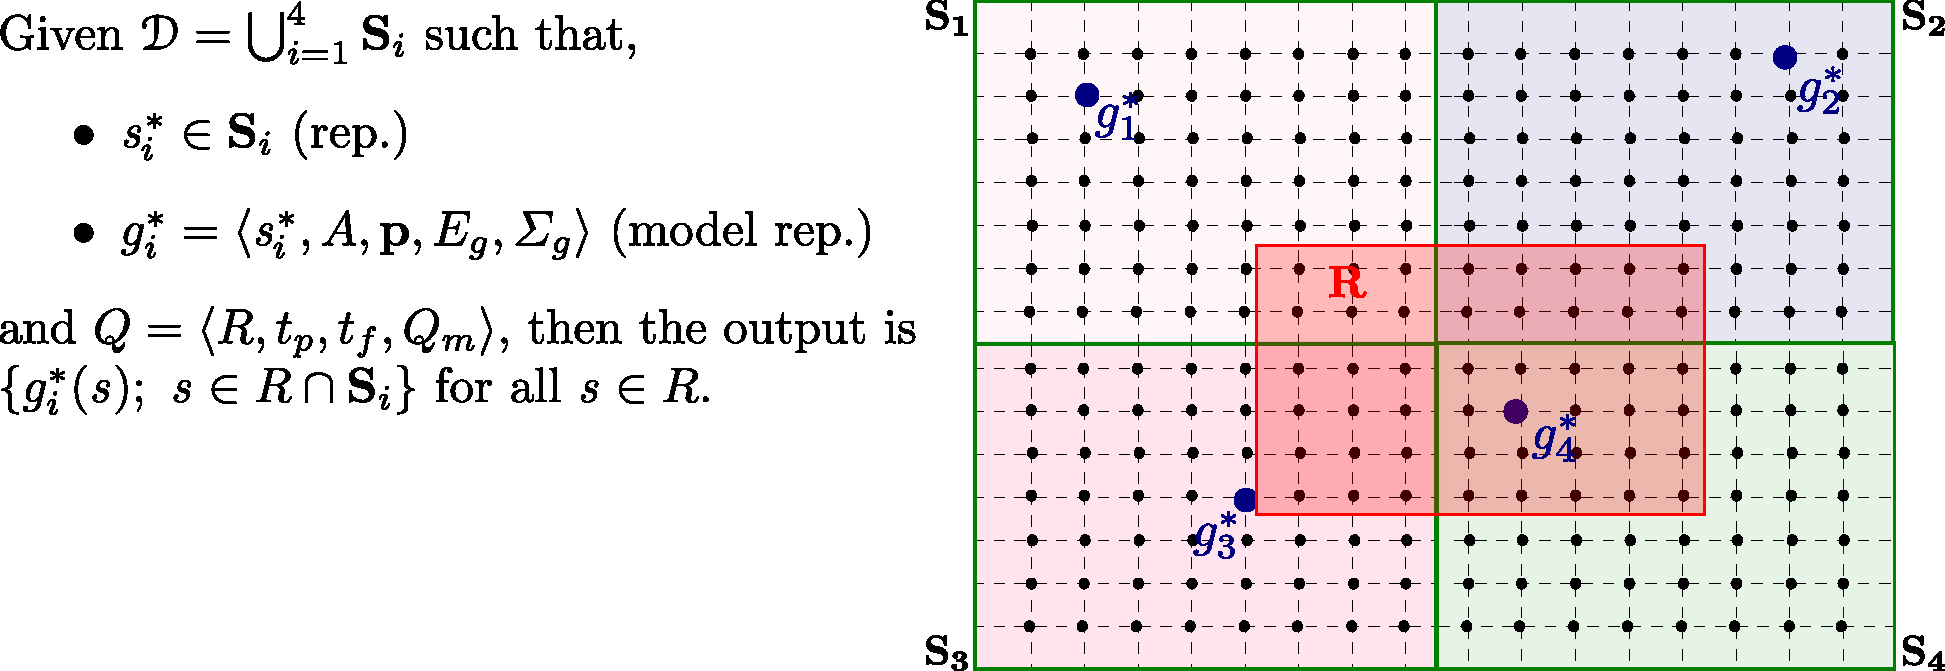
\includegraphics[scale=0.35]{../Figures/ModelComposition}
	    \caption{Model Composition using the Representative for a Region $\mathbf{S_{i}}$.}
	    \label{Fig:ModelRegion}
    \end{figure}

	\item Model Composition with Maximum Error: for each group, we find the time series for which its predictive model, when applied to all points of its corresponding group, maximizes the accumulated forecast error. It can be considered the `worst' choice for representatives. Together with the Minimal Error, it provides an interval that helps to quantify the appropriateness of the choice of representatives when using the `Model Composition of Representative Predictive Models'.
\end{itemize}

%TODO Describe products
As discussed in the previous section, in our problem, we are not considering a unique $k$ to analyze our methodology because there is no specific way to optimize the value of $k$. In the following section, we describe building a model composition that can leverage several given partitioning schemes.

% \subsection{Preparing a Classifier for Model Selection}
% \label{Sec:Classifier}

% In this section and the next, we seek to implement a process that can select models using some intelligence to find a composition of models to predict a region of interest with increased accuracy. The justification to implement this step is based on the intrinsic properties of the spatio-temporal data, the consistency and auto-correlation on nearby points in the domain makes difficult the task of finding an 'optimal' number of groups ($k$). Even when we consider the elements only in the temporal dimension, this difficulty persists \cite{Aghabozorgi2015}. In this step, our hypothesis consists in assuming that, if the predictive models on the representatives manage to predict a group of elements (prediction with a certain degree of confidence), based on the similarity of temporal patterns, these models will allow us to reach a prediction for a region of interest of the domain, in which we have only limited information about its past. 

% %Introducir la idea del clasificador o porque considero este 
% %For now, the desired output  of the classifier is expressed as follows: given a known time series, we want to find a representative among many different partitioning schemes, for which its predictive model can produce an adequate forecast.
% For now, the desired output of this step could be expressed as follows: given a known time series, we want to find a representative among many different partitioning schemes, for which its predictive model can produce an adequate forecast.

% Here, it is necessary to remember that, when computing the future value of a variable for a time series, we have to consider a range of values in the immediate past\cite{Chatfield2001}. Thus, to create a process for selecting models, we need a mechanism that allows us to find and use relationships between the set of representatives and past temporal instances of every element in the region of interest.

% We formulate this step as a univariate time series multi-class classification problem: Given an unlabeled univariate time series, assign it to one or more predefined classes. We consider the classes to be the identifiers of models computed at the representatives for each cluster. The time series takes part whenever multiple clustering is applied to the domain dataset. Thus, if a time series participates of two clusters, with $k_1$ and $k_2$ respectively, it would have associated two models $g_1$ and $g_2$ as labels. The label is composed with the value $k$ and the group index \texttt{cluster\_index} (c.i) where $0 \leq c.i <k$.

% In order to show how we can leverage domain partitioning schemes and their respective representatives, we use the formal representation of the problem (see Section \ref{Sec:ProblemFormalization}). With three different domain partitioning schemes as an example: Given three domain partitioning schemes for a spatio-temporal domain of sizes $m, n$ and $l$ and their respective representative sets, we have:
% \begin{eqnarray} 
% \nonumber
% \mathcal{D}	& = & \bigcup_{i=1}^{m} \mathbf{P_i} \,\,\textrm{and} \,\, \left\{\mathcal{P}_{1}, \ldots, \mathcal{P}_{m}\right\}, \\ \nonumber
% \mathcal{D} & = & \bigcup_{j=1}^{n} \mathbf{Q_j} \,\,\textrm{and} \,\, \left\{\mathcal{Q}_{1}, \ldots, \mathcal{Q}_{n}\right\}, \\ \nonumber 
% \mathcal{D} & = & \bigcup_{k=1}^{l} \mathbf{T_k} \,\,\textrm{and} \,\, \left\{\mathcal{T}_{1}, \ldots, \mathcal{T}_{l}\right\},
% \end{eqnarray}

% where $m, n, l < \textrm{card}(\mathcal{D})$. The set of representatives on the partitioning schemes considered is $\mathbf{R} = \left\{\mathcal{P}_{i}, \ldots, \mathcal{P}_{m}, \mathcal{Q}_{1}, \ldots, \mathcal{Q}_{n}, \mathcal{T}_{1}, \ldots \mathcal{T}_{l} \right\}$ , and $\mathcal{G}_{(\mathbf{R})}$ is the set of their correspondent models. Now, for an arbitrary element $\mathcal{S}$ in the domain, we want to find a representative $\mathcal{\hat{S}} \in \mathbf{R}$ of some group in a partitioning scheme, so that satisfies some optimization condition. Here we consider the representative $\mathcal{\hat{S}}$ such that has the minimum DTW distance with $\mathcal{S}$:

% \begin{equation}\label{eq:timeseries-representative}
%  \exists\, \mathcal{\hat{S}} \in \mathbf{R}, \,\, \textrm{such that}, \,\, \argminA_{\substack{\mathcal{\hat{S}} \in \mathbf{R}\\\mathcal{S} \in \mathcal{D}}} d_{DTW}(\mathcal{\hat{S}}, \mathcal{S}).
% \end{equation}

% In order to simplify the notation of the aforementioned relationship (\ref{eq:timeseries-representative}), we denote the representative with a label \texttt{[number\_of\_clusters, cluster\_index]}. Assuming that only the number of clusters is used as a parameter for partitioning schemes, this label can uniquely identify each of the representative models to extract a 'Time Series Classification Dataset ($TSCD$)`, similar to Table \ref{Tab:TSClassificationDataset}.

% \begin{table}[h]
% 	\centering
% 	%	\tiny
% 	\begin{tabular}{|c|c|}
% 		\hline
% 		Time-Series & Label for the Representative Model\\ \hline
% 		$\mathcal{S}_{1}$ & \texttt{[m, 1]} \\ \hline
% 		$\mathcal{S}_{2}$ & \texttt{[l, l-1]} \\ \hline
% 		$\mathcal{S}_{3}$ & \texttt{[n, n-2]} \\ \hline
% 		$\mathcal{S}_{4}$ & \texttt{[l, 2]} \\ \hline
% 		$\mathcal{S}_{5}$ & \texttt{[m, m-1]} \\ \hline
% 		$\vdots$ & $\vdots$ \\ \hline
% 	\end{tabular}
% 	\caption{Dataset of time series and labels satisfying relationship (\ref{eq:timeseries-representative}) for domain partitioning sizes $(m,n,l)$.}
% 	\label{Tab:TSClassificationDataset}
% \end{table}

% \subsection{Training a Classifier for Model Selection}
% \label{Sec:TrainingClassifier}

% % Idea of Classifier
% For the second part of the model selection process, we are interested in implementing a mechanism based on the knowledge acquired on an extracted dataset $TSCD$ (Table \ref{Tab:TSClassificationDataset}). The objective is, given a previously unseen time series, to infer a suitable label (and thus a predictive model on a representative) for it by recognizing patterns in the time series. It can be formulated as a time-series classification problem, which consists of training a classifier on a dataset $TSCD$ in order to map from the space of possible inputs to a probability distribution over the class variable values (labels).  

% With the proposed classification method, we will be able to learn from data about the membership relation between elements of the domain and representatives, and then use this learned knowledge to classify new time series. A dataset $TSCD=\{(\mathcal{S}_1,y_1),(\mathcal{S}_2,y_2), \ldots ,(\mathcal{S}_N,y_N)\}$ is a collection of pairs $(\mathcal{S}_i,y_i)$ where $\mathcal{S}_i$ is univariate time series with $y_i$ as its corresponding one-hot label vector of the labels \cite{Gulli2017}. For a dataset containing $m+n+l$ classes, the one-hot label vector $y_i$ is a vector of length $m+n+l$ where each element $j \in [1,(m+n+l)]$ is equal to 1 if the class of $X_i$ is $j$ and $0$ otherwise \cite{Mitsa2010}.

% % Multiclass classifier
% The task of time series classification is not a simple one. Considering the sequential aspect of time series data requires the development of algorithms that can harness this temporal property to select a class label from among a collection of candidates. While many neural network architectures can solve this problem, some work better than others \cite{Bagnall2017a}.

% In this work, we use Convolutional Neural Networks (CNNs). They typically fare very well on multiclass classification tasks, especially for images and text \cite{Goodfellow2016}. The powerful learning ability of deep CNN is primarily due to multiple feature extraction stages that can automatically learn representations from the data. Research has shown that using CNNs for time series classification has several advantages over other methods; they are highly noise-resistant models. They can extract very informative, deep features independent of time \cite{Wang2016, Bagnall2017a, Zhao2017}.

% % https://monkcage.github.io/blog/ai/2019/01/28/time_series_forecast.html
% % CNN-LSTM for Time Series Classification
% Another architecture is the Long-Short Term Memory Neural Networks (LSTM). The benefit of this model is that it can support very long input sequences. By implementing a hybrid CNN-LSTM Neural Network, we can integrate the capacity of process time series as blocks or sub-sequences by the CNN model, then pieced together by the LSTM model. Then the model will further divide each sample into further sub-sequences. The CNN model will interpret each sub-sequence, and the LSTM will piece together the interpretations from the sub-sequences. 

% % TODO we got what we wanted, a system that can receive a time series as input, and return a representative model as output.

\section{Step 4: Spatio-Temporal Predictive Query Processing}
\label{Sec:SpatioTemporalQueryProcessing}	

% $R = \langle R, t_p, t_f, Q_{m} \rangle$
In this section, we describe the on-line process implemented to compute a spatio-temporal predictive query, denoted in Equation \ref{eq:predictivequery}, (see Section \ref{Sec:ProblemFormalization}). The workflow of this process is shown in Figure \ref{Fig:OnLineQP}, and described as follows: 

\begin{figure}[!ht]
	\centering
	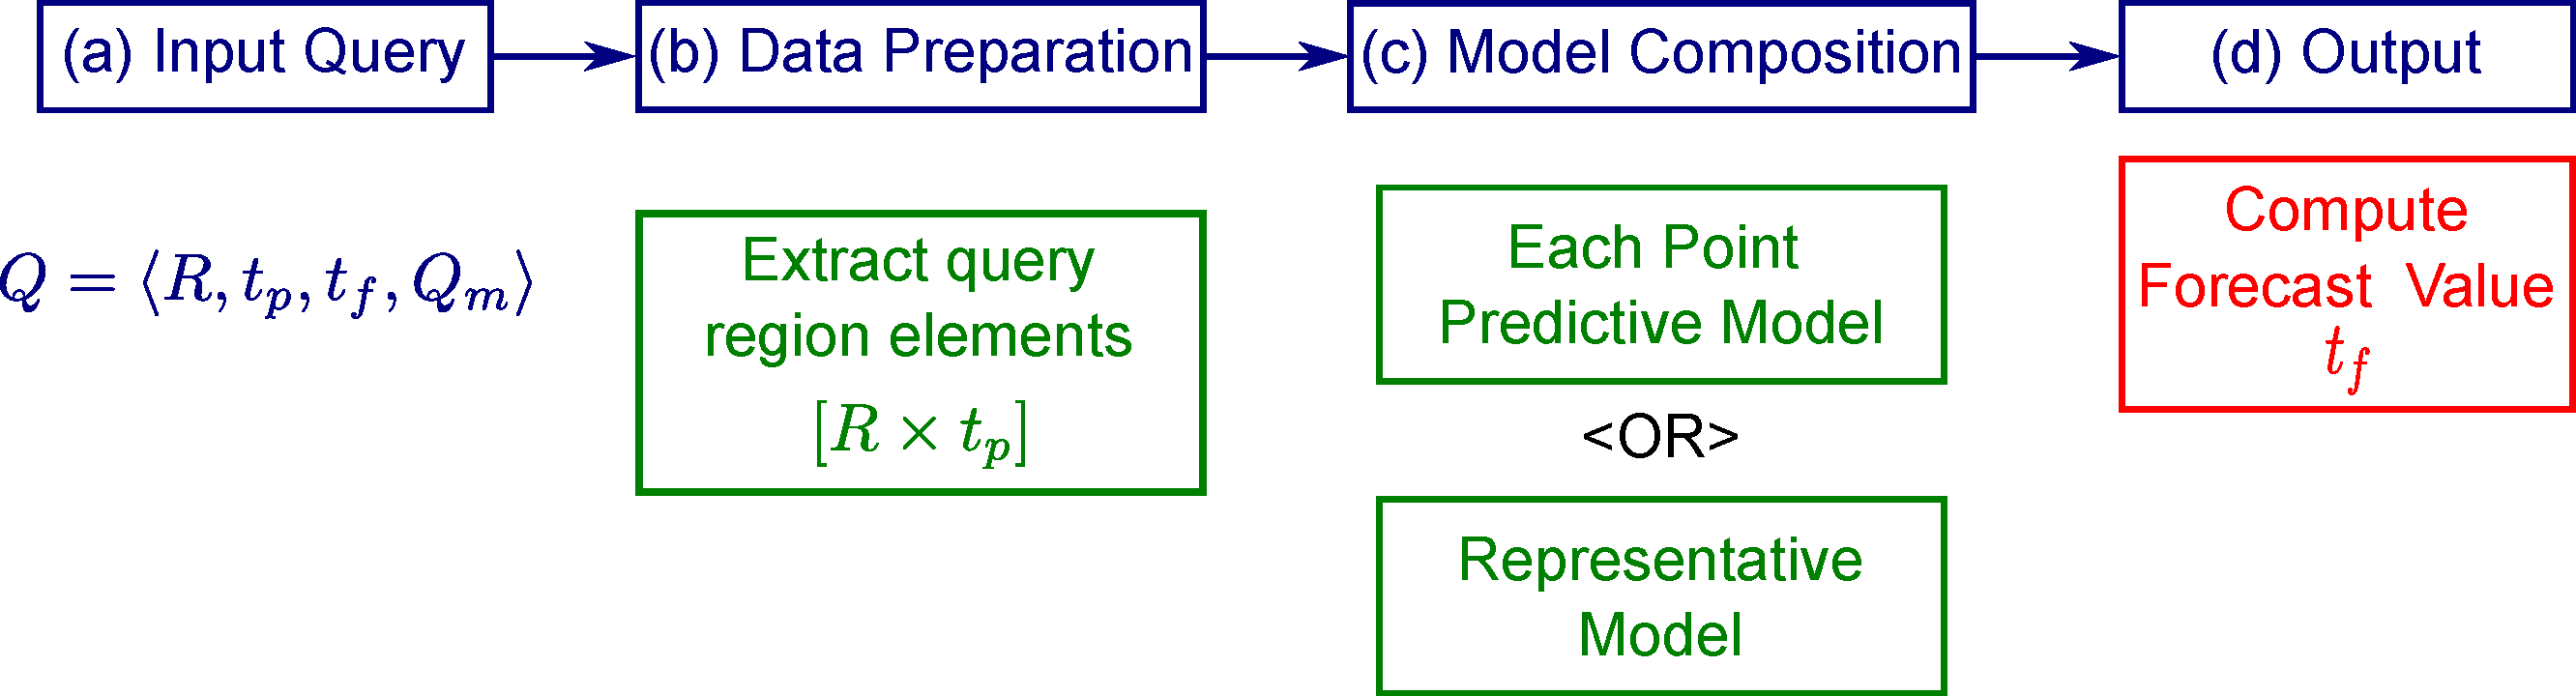
\includegraphics[scale=0.35]{../Figures/Query_Processing_Corrections}
	\caption{On-Line Processing Spatio-Temporal Predictive Query}
	\label{Fig:OnLineQP}
\end{figure}

\begin{itemize}
 \item [(a)] The input query is processed to extract the query region $R$ and the number of steps $t_p$ (past) and $t_f$ (future).
 \item [(b)] A data validation and extraction from the original dataset are performed according to the input parameters. The data processing for the query consists of the extraction of instances for the query region $R$ joint with past time units $t_{p}$, which means that for each point in $R$ exists a univariate time-series with $t_{p}$ values.
 \item [(c)] When processing a spatio-temporal predictive query, initially, we need to determine, for each point in the query region, which predictive models will be used. The model composition is then the resulting set of predictive models used to answer the predictive query with a forecast over the region of interest $R$. 
 
 Here, we implement two types of model composition for analysis, represented in Algorithm \ref{alg:modelcomp}. Note that we reuse terms from Section \ref{Sec:KnowledgExtraction}. It is done on purpose as the procedure for the model composition is the same but now limited to the subset region $R$. The three model compositions are described as follows:

 \begin{itemize}
	\item Model Composition with Point Predictive Models: For every point in the region of interest $R$, we use a baseline approach to train a predictive model on each point. To compute the forecast and associated forecast error, we use the model on each point.

	\item Model Composition of Representative Predictive Models: This approach uses the stored information corresponding to the domain partitioning schemes and their respective models. In this type of composition, we require a domain partitioning scheme (size $k$) specified as input of the query. Then, we identify the representatives for every point in the query region to load the predictive models that have been previously trained at the representatives. For each point in $R$, the model associated with its representative is used to compute the forecast and associated forecast error.
	
\begin{algorithm}[h!]
\caption{Load a Model Composition}\label{alg:modelcomp}
\begin{algorithmic}[1] 
\Function{load\_composition} {$D, comp\_id, t\_p$}

\State {$model\_comp\ \gets \bot$}

/* Model Composition with Point Predictive Models */
\If {$is\_point\_composition(comp\_id)$}

    
    /* Let model at each element predict its own element */
    \State{$model\_comp\ \gets load\_trained\_models\_each(D, t\_p)$}
    
\EndIf

/* Model Composition of Representative Predictive Models */
\If {$is\_representative\_composition(comp\_id)$}

    /* User needs to supply value for k of partitioning scheme */
    \State{$k\ \gets get\_k\_for\_request(comp\_id)$}
    
    /* Retrieve previously trained models at each representative */
    \State {$(medoids\_with\_models, D\_part)\ \leftarrow\ load\_models\_at\_medoids(D, k, t\_p)$}
    
    \For{$m \in medoids\_with\_models$}
    
        /* Retrieve the elements associated to current representative */
        \State {$cluster\ \gets elements\_represented\_by(m, D\_part)$}
        
        /* Let model at current representative predict these elements */
        \State{$model\_comp\ \gets set\_predictor(cluster, m, model\_comp)$}
    \EndFor

\EndIf

% \If {$is\_classifier\_composition(comp\_id)$}

%     /* Retrieve previously trained classifier */
%     \State{$classifier\ \gets load\_trained\_classifier(comp\_id, t\_p)$}
    
%     /* Classifier uses multiple partitioning schemes */
%     \For{$k \in classifier.k\_list$}
    
%         /* Retrieve previously trained models at each representative of current k */
%         \State {$(medoids\_with\_models, D\_part)\ \leftarrow\ load\_models\_at\_medoids(D, k, t\_p)$}

%         \For{$m \in medoids\_with\_models$}
        
%             /* Determine label associated to current representative */
%             \State {$medoid\_label\ \gets label\_for\_medoid(k, m, classifier)$}
            
%             /* Let model at current representative predict elements that match label */
%             \State{$model\_comp\ \gets assign\_predictor(medoid\_label, m, model\_comp)$}
%         \EndFor

%     \EndFor
% \EndIf

\State {$Return \ model\_comp$}
\EndFunction 
\end{algorithmic} 
\end{algorithm}
% 	\item Composition of Classifier for Predictive Models: The solver that calculates the result of a prediction query using the outcome of the time series classifier developed in Section \ref{Sec:TrainingClassifier}. The classifier is a function that, given an input series of size $t_p$, a predetermined suite of partitioning schemes, and a region, returns one of the representatives from any of the partitioning schemes available in the suite. Once the representative is determined, we follow the procedure for the `Model Composition of Representative Predictive Models' described in Section \ref{Sec:KnowledgExtraction}, but limited to the subset region $R$. It is the main model composition that we wish to evaluate, while the other two are presented for comparisons.
\end{itemize}
 
 \item [(d)] With the predictive models obtained from one of the model compositions of the previous step, the requested forecast for the $t_{f}$ steps for each point in $R$ is computed. 
 
 Additionally, if there is information available regarding the actual values of the predictive variable matching the forecast interval, the corresponding error is computed. Otherwise, the in-sample error of the model is used. Finally, the errors of the points in $R$ are combined using MSE (see Section \ref{Sec:ErrorTSA}) to produce a single scalar metric for the prediction error over $R$.
\end{itemize}

\begin{algorithm}[h!]
\caption{Process Online Predictive Query}\label{alg:online}
\begin{algorithmic}[1] 
\Function{processQuery} {$D, R, t\_p, t\_f, comp\_id $}

/* Choose a model composition, also load available models /*
\State {$model\_comp\ \gets load\_composition(D, comp\_id)$}

/* Extract $t\_p$ past time units for region $R$ /*
\State {$region\_data\ \gets extract\_region(D, R, t\_p)$}

\State {$query\_out\ \gets \bot$}

\For{$element\ \in\ region\_data$}

 /* model composition determines representative (medoid) to use /*
 \State {$representative\ \gets find\_repr(model\_comp, element)$}
 
 /* representative has trained model, do forecast of $t\_f$ steps /*
 \State{$forecast \gets predict(representative.model, element, t\_f)$}
 
 /* annotate the current element with forecast series and known error /*
 \State{$error \gets representative.error$} 
 \State {$annotate(element, forecast, error) $}
 
 /* the query result has a set of the annotated elements in R /*
 \State{$query\_result \gets add\_element(element, query\_out)$}
\EndFor

/* Compute the MSE of the errors for a single error metric over R /*
\State{$error\_mse \gets combine\_errors\_mse(query\_out)$}
\State {$annotate(query\_out, error\_mse) $}

/* Output is the forecast and error at each element of R, as well as the MSE /* 
\State {$Return \ query\_out$} 
\EndFunction 
\end{algorithmic} 
\end{algorithm} 

This online procedure described in this section can also be represented in Algorithm \ref{alg:online}. As input, the procedure takes the domain, the query parameters, and the type of model composition listed above. Then, for each element in the query region, the model performs the forecast, and the known in-sample error of the model is attributed. Finally, the MSE of the error is computed to produce the complete query output.

\section{Final Considerations}
\label{Sec:MethodologySummary}

This chapter describes the workflow for the proposed methodology, which is divided into an offline and an online phase. A domain partitioning technique is used to obtain domain representatives and groups during the offline phase, then predictive models for these representatives are generated. A time series classification approach is also considered for model selection. The decision to include such a classifier will be justified with experimental results that explore the predictive accuracy when using different partitioning schemes. Finally, the online phase represents the execution of a spatio-temporal predictive query. We thoroughly describe the methods and techniques used for each of these steps, highlighting the available choices and baseline comparisons. We also present pseudo-code of algorithms that summarize the main aspects of each phase.